\chapter{Marco Teórico}

 En este capítulo se aborda el marco teórico necesario para comprender más fácilmente el desarrollo de los capítulos posteriores. Se analiza el problema del tráfico en general y soluciones como la construcción de corredores exclusivos para el transporte público. En este contexto se detalla el Corredor de Garzón tanto su descripción como sus problemas. Luego se da un breve repaso sobre los simuladores de tráfico y la teoría detrás de los algoritmos evolutivos. Para finalizar se encuentra una lista con trabajos relacionados para mostrar otras soluciones y variantes.

\section{Problema del tránsito vehicular}

En gran parte del mundo se está produciendo un crecimiento sostenido del parque automotor, esto ocasiona una serie de problemas relacionados con el agravamiento de las congestiones vehiculares que afectan la calidad de vida de las personas.  \citep{Cepal2003}.

Este problema tiene un gran impacto en el desarrollo de las ciudades por lo que es un componente principal en los planes estratégicos para su crecimiento.

La congestión ocasiona una progresiva merma de la velocidad promedio de circulación. Esto provoca un incremento en la duración de los viajes y del consumo de combustible. Esto repercute en la contaminación atmosférica y sonora que directamente la salud de las personas, además se genera una exigencia en las vías de tránsito que ocasiona un deterioro mayor de calles y rutas.

Uruguay no escapa a este fenómeno, en particular Montevideo, donde el aumento del parque automotor está en ascenso constante desde el 2005 \citep{INE2014}.
Y según proyecciones el crecimiento seguiría en un promedio de 4.5\% anual hasta el 2020. \citep{BBVA2013}

Esto viene de la mano con el sostenido aumento de las ventas de vehículos  desde el 2003 \citep{Autoanuario2014}

\begin{figure}[H]
	\centering
	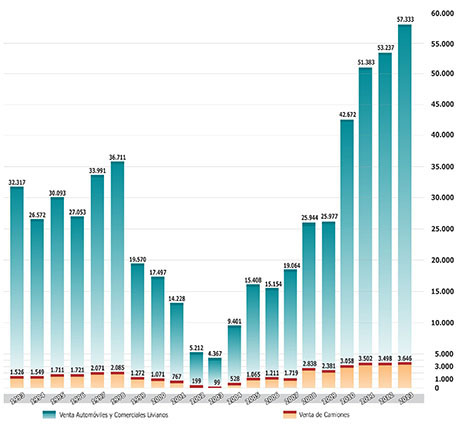
\includegraphics[width=0.9\linewidth]{Figures/ventas_autos}
	\caption{Evolución en la venta de automóviles por año. El valor mas bajo corresponde al año 2003, y el mas alto 2013. Imagen extraída de \citet{Autoanuario2014}.	
	}
	\label{fig:ventas_autos}
\end{figure}


Los expertos indican que la congestión ya está instalada y la infraestructura vial no acompasó este crecimiento. Montevideo es la ciudad con más semáforos por automóvil en Latinoamérica, con más de 620 cruces semaforizados, alguno de los cuales no están coordinados.\citep{Subrayado2013}

En un contexto global el crecimiento en la circulación de automóviles provoca que baje el nivel de aceptación del transporte público cuyo servicio en general es ineficiente. Para resolver este problema las autoridades suelen optar por sistemas de transporte costosos como los \emph{metros} pero se ha demostrado que existen otras opciones viables como el BRT (Bus Rapid Transit / ómnibus de tránsito rápido)\citep{BRT_Dial}.

En el caso de Montevideo para solucionar este problema se está implementando el plan de movilidad urbana \citep{PlanMovilidad} con el objetivo de mejorar la eficiencia del transporte público y democratizar el acceso al mismo. El sistema de transporte está inspirado en un BRT con la construcción de varios corredores exclusivos en la ciudad. En la siguiente sección se dará más información sobre los BRT, corredores urbanos y en particular el Corredor de Garzón.



\section{Corredores urbanos de tráfico}

El corredor urbano de tráfico o también llamado corredor segregado se caracteriza por una separación física entre el carril de circulación de los ómnibus y los carriles para el resto del tráfico. 
Esta es la principal diferencia con un concepto similar llamado \emph{carril de sólo bus} en donde se separan por líneas horizontales pintadas en la calle indicando que sólo pueden circular ómnibus. Los carriles de \emph{sólo bus} suelen fracasar por falta de control que evite que el tráfico los invada. En el caso de Montevideo el carril \emph{sólo bus} está sobre la derecha, por lo que los vehículos privados lo invaden al virar a la derecha y lo mismo los taxis para levantar pasajeros. Al hacer los corredores alineados en el medio del tráfico se evitan esos problemas.  

Las ciudades de países en vías de desarrollo deben estudiar si pueden instalar corredores pues son fundamentales para conseguir mayores velocidades en el sistema. Pero hay muchas posibilidades y no todas pueden ser aplicables por el contexto zonal, cultural o de inversión necesaria.

\begin{figure}[H]
	\centering
	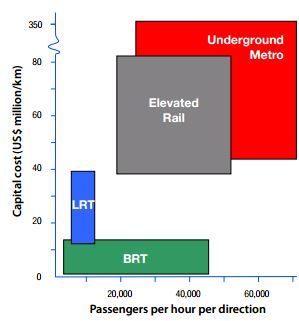
\includegraphics[width=0.5\linewidth]{Figures/costo_transporte}
	\caption{Gráfica de costos de transporte en función de la gente transportada. En el eje horizontal esta la cantidad de pasajeros por hora, en el vertical el costo en millones de dólares por kilómetro.  BRT (Bus Rapid Transit), LRT(Light Rail Train)- Imagen original extraída de \citep{ITDP}		
	}
	\label{fig:Grafica de costos de otros medios de transporte}
\end{figure}

Bus Rapid Transit (BRT) es una solución innovadora, de alta capacidad y de menor costo para el transporte público que puede alcanzar el rendimiento y los beneficios de modos ferroviarios con un costo significativamente menor. Se trata de un sistema integrado de movilidad basado en ómnibus para el transporte de los pasajeros a sus destinos de manera rápida y eficiente. Al mismo tiempo ofrece la flexibilidad necesaria para satisfacer una variedad de condiciones locales. Los elementos del sistema de BRT pueden ser fácilmente personalizados a las necesidades de la comunidad e incorporan tecnologías de última generación de bajo costo que atraen a más pasajeros y en última instancia ayudan a reducir la congestión de tráfico en general.

Un BRT contiene características similares a un tren ligero o el sistema de metro por ese motivo es mucho más confiable, conveniente y más rápido que los servicios regulares de ómnibus. Con las características adecuadas, el BRT es capaz de evitar las causas de los retrasos que suelen tener los servicios regulares de ómnibus, como estar atrapado en el tráfico y hacer cola para pagar a bordo. 


	
\section{Corredor de Garzón}	


Fue construido como parte del plan de movilidad urbana que incluye otros corredores en la ciudad de Montevideo. \citep{PlanMovilidad}. Tomando en cuenta sus extremos conecta los barrios de Colón con Paso Molino. Tiene una extensión de 6.5km con 24 cruces semaforizados, en donde se encuentran calles importantes como Millán que conecta con una autopista (Ruta 5) y Bulevar Batlle y Ordoñez la cual tiene una gran densidad de tráfico. Es importante aclarar que no es sólo una conexión de extremo a extremo ya que se encuentra en una zona densamente poblada cuyos barrios tienen al corredor como la principal vía de movilidad.

\begin{figure}[H]
	\centering
	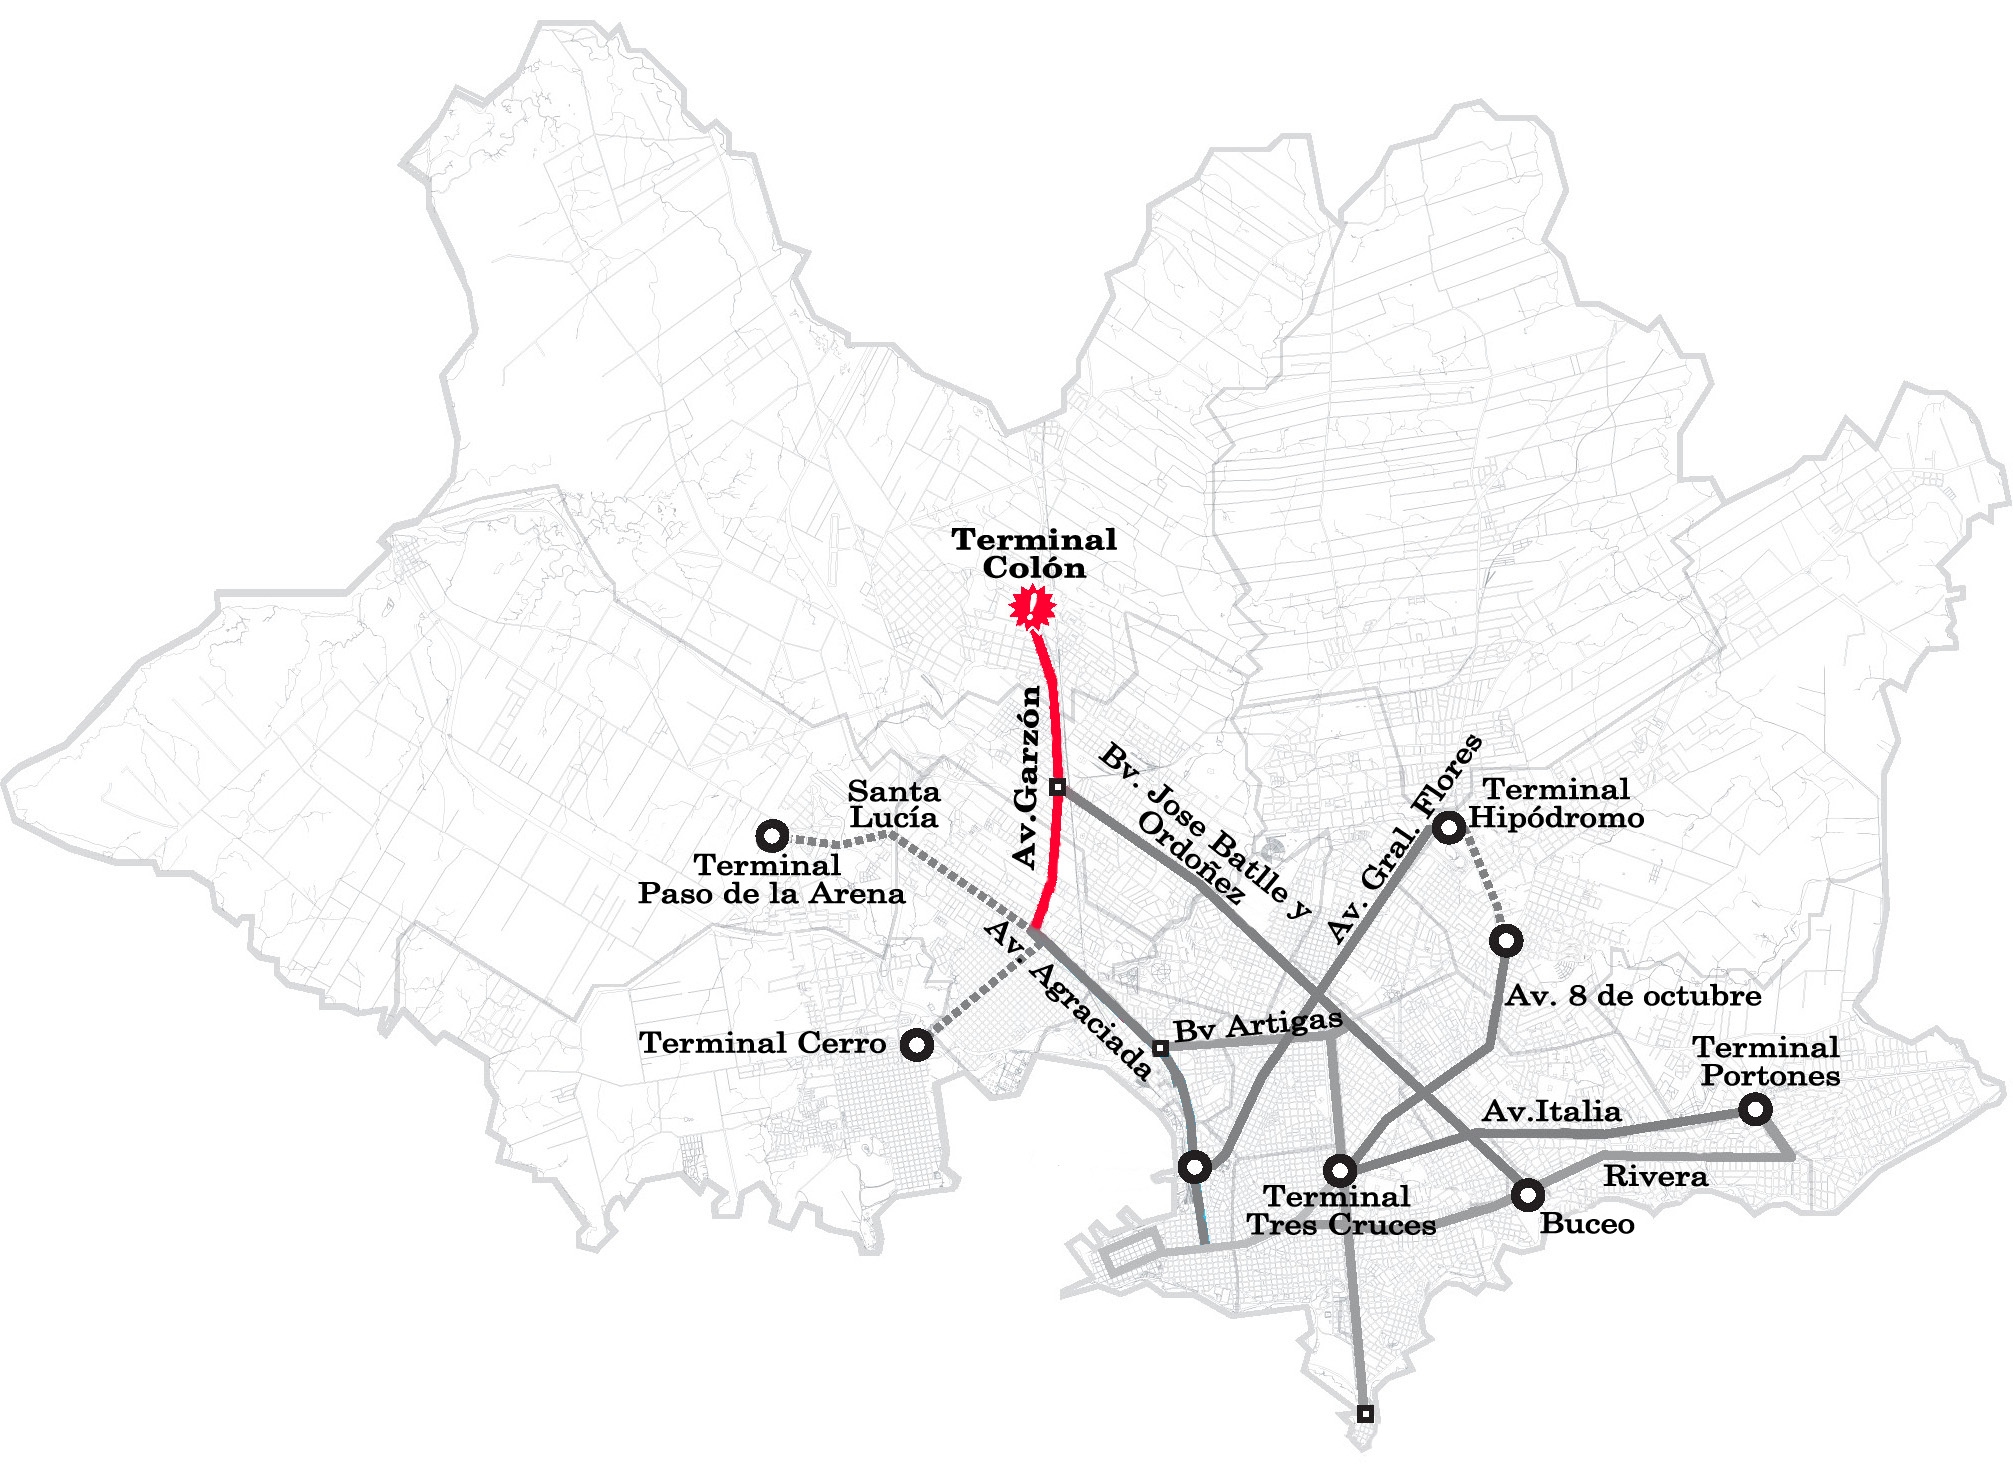
\includegraphics[width=0.7\linewidth]{Figures/Mapa_Garzon_0}
	\caption{Localización del Corredor de Garzón en Montevideo - Imagen original extraída de www.montevideo.gub.uy		
	}
	\label{fig:Grafica de costos de otros medios de transporte}
\end{figure}

Como se aprecia en la figura \ref{fig:perfil_garzon} el corredor consiste básicamente de tres calles paralelas e independientes; dos de ellas con dos carriles de una sola mano y entre medio de éstas se encuentra una calle doble vía con un carril para cada vía que es exclusivamente usado por ómnibus urbanos durante el día y también por suburbanos en la noche.


Basándonos en el standard antes mencionado, el Corredor de Garzón cumple con la definición de BRT por los siguientes puntos:
\begin{itemize}
	\item Largo mínimo del corredor. 3 km de corredor exclusivo 
	\item Vía de ómnibus dedicada. Al tener un 90\% de segregación física dentro del corredor.
	\item Alineación de la vía del ómnibus. Por estar constituido por dos carriles centrales para el ómnibus en medio de los carriles de otros vehículos.
	\item Tratamiento de intersecciones. Por prohibir algunos virajes a la izquierda y el carril de ómnibus tener prioridad en la mayoría de las intersecciones.
\end{itemize}


Analizando las recomendaciones del standard hay algunas que no están totalmente aplicadas al corredor, entre ellas destacamos:

\begin{itemize}
	\item Cobrar el boleto fuera del ómnibus. Uno de los factores más importantes para mejorar la experiencia del usuario así como también la velocidad en zonas de mucha carga es que hayan al menos algunas estaciones (no solo paradas de ómnibus) donde el boleto se cobre al entrar a la estación o se cargue la tarjeta en su defecto.
	\item Servicios expresos o limitados. Una forma de mejorar las velocidades de operación consiste en crear líneas que no se detengan en todas las paradas, sobre todo salteen las de menor demanda así se podría mejorar la velocidad y poner más ómnibus en la calle.
	\item Carril extra para adelantarse en paradas. En sistemas de gran porte es crítico para poder manejar los servicios expresos, en sistemas de baja demanda es de igual manera una buena inversión y en el caso del corredor de Garzón podría permitir que los servicios suburbanos fueran todo el día por el corredor mejorando así el transporte público y privado.
	\item Distancia entre paradas e intersecciones. Según el standard, la mínima distancia entre la intersección y la parada es de 26m pero idealmente deberían ser 40m para evitar retrasos. En el Corredor de Garzón las paradas están sobre las intersecciones y hay varias donde se detiene más de una línea de ómnibus. Esto puede ocasionar problemas porque mientras uno o dos ómnibus ya realizaron la parada y esperan por el semáforo, los demás que lleguen generaran una fila aguardando por detenerse en la parada para levantar a los pasajeros y posiblemente luego, cuando lleguen al cruce no tendrían la luz verde.
	\item Tener estaciones centrales o conexión entre paradas. Que la parada no se encuentre en el centro de los dos carriles de ómnibus, hace que sea una construcción más cara (hay que hacer dos paradas) y el hecho de que no haya una conexión física por la cual el pasajero pueda cambiar de recorrido de un lado al otro sin tener que cruzar la calle, lo hace menos eficiente y más inseguro.
	\item Distancia entre estaciones.  Las paradas deberían de estar a una distancia de entre 300m y 800m, siendo 450m el óptimo tanto para el pasajero como el transporte.
	\item Puertas de los ómnibus. Tener dos puertas anchas o más de tres puertas comunes. Que los pasajeros puedan entrar y salir por todas ellas permite un mayor flujo y volumen de gente transportada.
	\item Semáforos. Un corredor debe de funcionar al igual que una autopista en el sentido de que una vez que se entra debería ser posible mantener la velocidad máxima sin tener que detenerse seguido, por lo que no deberían de haber semáforos cerca uno de otro, de haberlos la sincronización será la clave para minimizar los tiempos de espera.
	\item Calles paralelas. Tener calles paralelas es de vital importancia para un corredor ya que una de las formas de minimizar los tiempos de espera es prohibir los giros a la izquierda, y una calle paralela provee la facilidad de poder realizarlo.
	\item Giro a la derecha con luz roja. Actualmente en muchos países se encuentra reglamentada una ley que permite a los conductores doblar a la derecha con luz roja ya que la misma (a menos que se especifique) es tomada como un cartel de pare \emph{solamente} para doblar a la derecha. Esta ley en donde esta aprobada acorta los tiempos de luz verde de las transversales mejorando así la velocidad promedio en los corredores o calles importantes.
	\item Mejor calidad de estaciones. Que las paradas sean a prueba del clima, con puertas corredizas que abren cuando hay un ómnibus (para que nadie caiga al corredor), con información al pasajero en tiempo real, etc. No harían al corredor más rápido pero si más seguro, cómodo y confiable.
\end{itemize}


\begin{figure}[H]
	\centering
	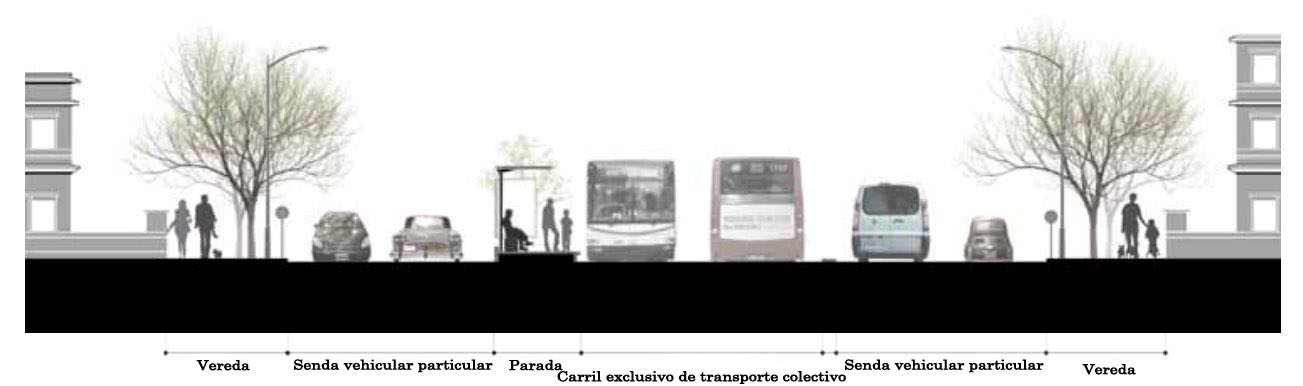
\includegraphics[width=0.9\linewidth]{Figures/busway_configuration}
	\caption{Perfil propuesto para el corredor Garzón desde San Quintín a Camino Colman - Imagen original extraída de \citep{PlanMovilidad}
	}
	\label{fig:perfil_garzon}
\end{figure}

Desde su construcción el corredor ah recibido críticas debido a que su principal objetivo que era agilizar el transporte público no fue cumplido, luego de intentos de mejoras al respecto se ha vuelto a la velocidad promedio que existía antes de realizar el corredor para el transporte público \citep{olivera2015}.


Las autoridades han admitido que se han cometido errores y se apunta a que no se ha logrado sincronizar los semáforos.\citep{olivera2013}. Un buen funcionamiento de los mismos es fundamental para asegurar que el tráfico se mueva con eficiencia y a la vez aporte seguridad a los peatones. A continuación se tratará este tema. 


\section{Sincronización de semáforos}
El problema de la optimización del tráfico se refiere a los métodos cuyo objetivo es mejorar el flujo de vehículos en una red vial. Estos se pueden clasificar en dos categorías: influir en el comportamiento de los conductores (configuración de semáforos, señalización, etc) o modificaciones en las rutas (agregado de un nuevo carril, ensanchar calles, etc). 
Estos últimos pueden producir mejoras drásticas pero requieren una inversión monetaria y espacio físico que muchas veces no esta disponible. Por esta razón los métodos destinados a influir en el comportamiento de los conductores se presentan como una mejor o única opción.

En este sentido los métodos para la sincronización de semáforos son de los más efectivos para agilizar el tránsito y no generar congestiones, aumentando la velocidad promedio de los viajes y mejorando las perspectivas de desarrollo de la ciudad así como la calidad de vida de sus habitantes. 

La fase se refiere a una configuración especifica de luces de semáforos en una intersección, que permiten el movimiento de ciertos flujos de tráfico. Como se ve en la figura \ref{fig:fases} cada intersección puede tener diferente número de fases y también distintas duraciones. Estas suelen ser configuradas y establecidas manualmente por técnicos especializados basados en su experiencia, aunque en ciertas ocasiones se utilizan simulaciones para obtenerlas. 

\begin{figure}[H]
	\centering
	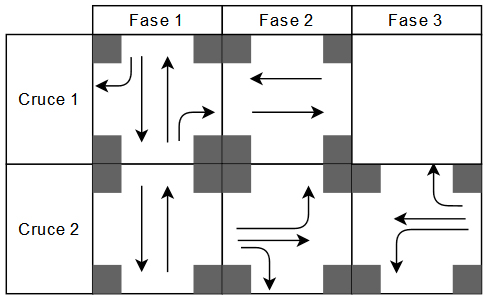
\includegraphics[width=0.8\linewidth]{Figures/fases1}
	\caption{Distintas fases para dos cruces en una red de tránsito}
	\label{fig:fases}
\end{figure}

Existen tres parámetros importantes a tener en cuenta que determinaran el comportamiento del sistema, estos son la duración de fase, los ciclos de las luces y los valores de \emph{offset}. Estos serán explicados a continuación.


\begin{itemize}
 	\item Duración de fase: Se refiere a la duración en que una configuración especifica de luces esta activa en una intersección. Un conjunto de ellas estará en verde y otras en rojo determinando quien cruza en ese momento. La elección correcta de este parámetro es fundamental, las calles con una densidad de tránsito mayor tendrían que tener más tiempo para cruzar. Destacar que realizar la optimización individual de estos cruces no tiene por que llevar a una solución optima en la red, ya que se pueden producir cambios en el flujo que afecten a las demás. Por esta razón hay que tener un enfoque global al realizar una solución.
 	
 	\item Duración del ciclo: Un ciclo representa un conjunto de fases, en general su duración es la suma de las duraciones de las fases. Como indica su nombre el ciclo se repetirá una vez se completa. La duración puede incrementarse o decrementarse para permitir mayor cantidad de repeticiones de las fases. Otro punto a considerar sobre todo en intersecciones complejas es el orden en el cual las fases son ejecutadas.
 	
 	\item Offset: Indica el comienzo de una fase permitiendo que diferentes intersecciones comiencen su ciclo en diferentes momentos, esto es muy importante para sincronizar un flujo de tráfico en lo que se conoce como \emph{línea verde}, en donde los vehículos logran pasar todas las intersecciones sin detenerse.
\end{itemize}

Estos parámetros pueden ser utilizados a la hora de sincronizar los semáforos de una zona, buscando una optimización global de la red. También hay que tener en cuenta el desarrollo de soluciones seguras siendo lo más básico que no existan intersecciones donde ambos flujos crucen a la misma vez.

Existen diversos métodos para lograr la coordinación necesaria que van desde simples mecanismos de reloj a sistemas computarizados que se ajustan en tiempo real con ayuda de sensores en la calle. Pudiendo clasificarse como estrategias de tiempo fijo, o de tiempo dinámico auto-ajustable.

Se considera a este problema en la categoría de NP-difícil, es decir que no existe hasta el momento un método determinístico que lo resuelva.

Existen diversos métodos computacionales para solucionar este problema alguno de los cuales se encuentran en la sección de trabajos relacionados. Entre los mas desarrollados y efectivos están los algoritmos evolutivos en particular los algoritmos genéticos que serán explicados a continuación.

\section{Algoritmos Evolutivos}

Los algoritmos evolutivos son un conjunto de técnicas heurísticas para la resolución de problemas complejos que se inspiran en la evolución natural, trabajan sobre una población de individuos que representan una solución y utilizan mecanismos de selección, reproducción y diversidad para lograr su objetivo. 
Es una técnica iterativa que busca en cada paso mejorar las soluciones por medio de operadores basado en un criterio predefinido a maximizar o minimizar.

Se pueden destacar cuatro etapas en la ejecucion del algoritmo evolutivo. Estos son:

\begin{itemize}
	\item Evaluación: Para cada individuo de la población se determina un valor de aptitud (fitness) en relación a su capacidad para resolver el problema. 
	\item Selección: Proceso en donde se eligen cuales son los individuos que sobrevivirán a la siguiente generación y sobre los cuales se aplicaran los operadores.
	\item Operaciones: Se aplican tanto combinaciones entre individuos (cruzamiento), como operadores de diversidad(mutación). Esto genera nuevos individuos en la población.
	\item Reemplazo: Se produce el recambio generacional, sustituyendo a la antigua población por una nueva que podría tener sobrevivientes de la anterior o solamente nuevos individuados generados en la etapa anterior.
\end{itemize}

Se han desarrollado varias lineas de investigación diferenciadas que aplican estas técnicas, alguna de ellas se describen a continuación:

\begin{itemize}

	\item Estrategias de Evolución: Propuesto por \citet{Ingo1971}, comenzó como un método de optimización utilizando individuos compuestos por números reales en problemas relacionados al diseño de ingeniera. Su característica principal es que utilizan el operador de mutación como motor para la evolución. Aunque modelos mas recientes agregan otro tipo de mecanismos.
	\item Programación genética: Intenta generar un programa de computación para resolver una tarea especifica. Cada individuo puede ser un programa que es representado en forma de árbol, de esta manera la combinación entre individuos se realiza de forma más sencilla. La función de aptitud se refiere a que tan cerca de resolver la tarea se encuentra el individuo.\citep{Koza1992}
	\item Algoritmos Genéticos: El mas popular de los algoritmos evolutivos, aplicado para resolver problemas de optimización. El operador de cruzamiento es el principal motor evolutivo siendo el de mutación el secundario. En la siguiente sección se darán mas detalles sobre los mismos.
\end{itemize}




\subsection{Algoritmos Genéticos}

La idea base es que partiendo de una población inicial de individuos se seleccionan los mejores en base a su aptitud respecto a solucionar el problema y estos se utilizan para generar nuevos individuos ya sea por combinación o modificación. Por tanto en cada paso obtenemos mejores soluciones hasta detenernos usando un criterio de parada, ya sea el número de iteraciones o cuando ya no se puede mejorar más la solución. Los trabajos de \citet{Goldberg1989} y \citet{Mitchell1996} brindan más detalles sobre los mismo.

Un individuo es una codificación de la solución que resuelve el problema. La población inicial puede generarse aleatoriamente o basándose en algún conocimiento previo. La función de evaluación o fitness indica que tan buena o apta es una solución en comparación con las demás.
En cada iteración la cual se conoce como generación se aplican operadores de cruzamiento, estos son formas de combinar a los individuos para obtener otros que potencialmente sean una mejor solución y también cambios aleatorios sobre los individuos llamado mutación.


\begin{figure}[H]
	\centering
	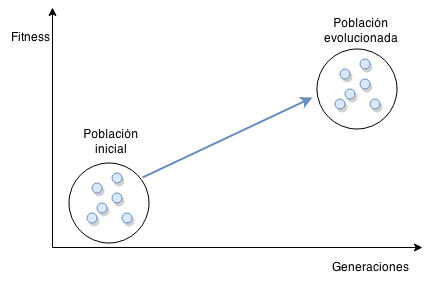
\includegraphics[width=8cm]{Figures/fitness_generaciones}
	\caption{La evolución se produce al mejorar el fitness de la población a lo largo de las generaciones.}
	\label{fig:fitness_generaciones}
\end{figure}



Por tanto se van seleccionando, combinando y cambiando las mejores soluciones en un proceso que va obteniendo mejores soluciones.
El criterio de parada nos indica cuando termina este proceso, ya sea por que se alcanzó un número de generaciones predefinidos o por que la mejora no es evidente. Al final se devuelve la mejor solución encontrada en todo el proceso.

Hay que indicar que no es una técnica exacta pero logra muy buenas aproximaciones, además es muy buena en problemas complejos por su flexibilidad y robustez. 


\subsubsection{Representación de soluciones}
No podemos trabajar directamente sobre las soluciones, por lo que tenemos que codificarlas en un modelo que nos sirva para poder aplicar el algoritmo.
La inspiración biológica se ve en los nombres que adopta esta representación, llamada Cromosoma que es un vector de genes y cada valor de un gen se llama alelo.
En general se codifica un vector de números binarios o reales de largo fijo, lo que facilita la aplicación de los operadores.

\begin{figure}[H]
	\centering
	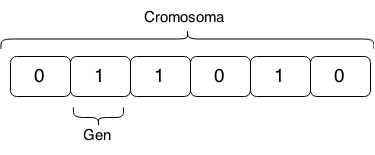
\includegraphics[width=8cm]{Figures/rep_binaria}
	\caption{Representación binaria de un cromosoma.}
	\label{fig:rep_binaria}
\end{figure}


\subsubsection{Función de Evaluación} 
Indica que tan bueno es un individuo para resolver el problema en cuestión con un valor conocido como Fitness. Este se utiliza para seleccionar a los mejores y de esta forma guiar la exploración hacia la mejor solución.
Se deben tener en cuenta las restricciones del problema para que las soluciones no factibles no sobrevivan.
En general es donde se consume el mayor tiempo del algoritmo en comparación con los demás operadores.

\subsubsection{Operador de Selección}
Existen diversos operadores de selección , su función es que las mejores características de los individuos se mantengan en las siguientes generaciones.
Los tipos más populares son:

\begin{itemize}
	\item Ruleta: También conocida como selección proporcional elige aleatoriamente individuos en la cual la probabilidad de selección es proporcional al valor de fitness.
	\item Torneo: Se elige aleatoriamente un determinado número de individuos los cuales compiten entre si usando su valor de fitness.
	\item Rango: Se ordenan los individuos por fitness y se seleccionan los mejores.
\end{itemize}

\subsubsection{Cruzamiento}
Su función es combinar individuos con el objetivo de preservar las mejores características y así lograr mejores soluciones. 
Existe una tasa que se puede modificar para indicar la probabilidad de que se realice el cruzamiento.

\begin{itemize}
	\item Cruzamiento de un punto: A partir de dos padres se selecciona un punto al azar de los cromosomas obteniendo dos trozos que se combinan para obtener dos hijos. Se explica en la figura ~\ref{fig:cruzamiento1}
	\item Cruzamiento multipunto: El método anterior se puede generalizar para obtener más puntos de corte y más recombinaciones.
\end{itemize}

\begin{figure}[h]
	\centering
	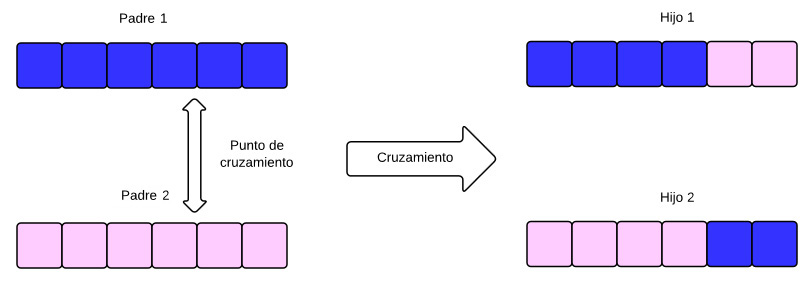
\includegraphics[width=\textwidth]{Figures/cruzamiento1}
	\caption{Cruzamiento de un punto}
	\label{fig:cruzamiento1}
\end{figure}

\subsubsection{Mutación} 
Indica el método utilizado para modificar un individuo, esto se realiza para lograr más diversidad y no caer en máximos locales. En general aplica una modificación aleatoria en el cromosoma.Hay una tasa de probabilidad para aplicar este operador que en general es muy baja. 
\begin{figure}[h]
	\centering
	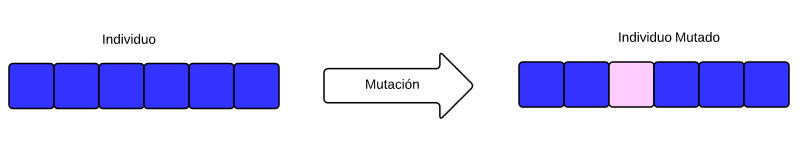
\includegraphics[width=1\linewidth]{Figures/mutacion1}
	\caption{Mutacion por inversión binaria}
	\label{fig:mutacion1}
\end{figure}


\subsubsection{Reemplazo} 
Luego de que se aplica el cruzamiento se insertan nuevos individuos que aumentan la población original por tanto este operador indica cual es el criterio que debemos tomar para crear una nueva población con una cantidad de individuos igual a la original.
Se podría reemplazar todos los padres por los hijos, o seleccionar cuales reemplazar, entre otros criterios.

\subsubsection{Criterio de parada} 
Indica cuando debe terminar el algoritmo, puede ser definiendo un número fijo de generaciones o analizando si el mejor valor de fitness se mantiene relativamente constante durante un número determinado de generaciones entre otros criterios. El objetivo será encontrar un compromiso entre un buen resultado y un tiempo acorde de ejecución, ya que el algoritmo no arrojara un valor exacto sino una buena aproximación. 

\subsubsection{Funcionamiento}

El esquema básico de funcionamiento es el siguiente:


\begin{algorithm}[H]
	\caption{Algoritmo Genético}
	\label{alg:algoritmo_genetico_simple}
	\begin{algorithmic} [1] 
		{
			%\small
			\STATE {Inicializo( Pob(0))}
			\STATE \texttt{generacion} = 0
			\WHILE {\text{No llegue al criterio de parada}}
			\STATE {Evaluar Pob(generacion)}
			\STATE {Padres = Seleccionar(Pob(generacion))}
			\STATE {Hijos = Cruzamiento(Padres) y Mutacion(Padres)}
			\STATE {NuevaPob = Reemplazar Pob(generacion) con Hijos}
			\STATE \texttt{generacion}++
			\ENDWHILE
			\RETURN Mejor solución
		}
	\end{algorithmic}
\end{algorithm}



% ctrl+t comenta
%\begin{algorithm}%[!ht]
%	\caption{Genetic Algorithm}
%
%	\begin{algorithmic} [1] 
%		{
%
%			\STATE {Init( Pop(0))}
%			\STATE \texttt{generation} = 0
%			\WHILE {\text{NOT Stop Criteria}}
%			\STATE {Evaluate Pop(generation)}
%			\STATE {Parents = Selection(Pop(generation))}
%			\STATE {Children = Crossover(Parents) and Mutation(Parents)}
%			\STATE {NewPop = Replace Pop(generation) with Children}
%			\STATE \texttt{generation}++
%			\ENDWHILE
%			\RETURN Best solution
%		}
%	\end{algorithmic}
%\end{algorithm}


\subsection{Algoritmos genético multiobjetivo}

Los problemas de optimización multiobjetivo trabajan sobre un espacio multidemensional de funciones y no tienen una única solución por esto el significado de optimo cambia. Una solución es un optimo de Pareto si ninguna de las funciones objetivos puede mejorar su valor sin degradar otro de los valores objetivos. Todas las soluciones de Pareto son consideras igualmente buenas ya que los vectores no se pueden ordenar completamente. Al conjunto de los valores funcionales de los óptimos de Pareto se les llama frente de Pareto.

Existen algoritmos evolutivos para resolver el problema de la optimización multiobjetivo estos son los llamados MOEA por sus siglas en ingles \emph{ MultiObjetive Evolutionary Algorithm}. Para un análisis más detallado se recomienda el trabajo de \citet{Deb2001}.

Lo que buscan es aproximarse al frente de Pareto y lograr mostrar una gama de diferentes compromisos entre las funciones a optimizar para luego poder tomar la decisión de cual elegir.


\begin{algorithm}%[!ht]
	\caption{Algoritmo Evolutivo MultiObjetivo. En rojo se indican las diferencias con el algoritmo evolutivo genérico.}
	\label{alg:algoritmo_genetico_multiobjetivo}
	\begin{algorithmic} [1] 
		{
			%\small
			\STATE {Inicializo( Pob(0))}
			\STATE \texttt{generacion} = 0
			\WHILE {\text{No llegue al criterio de parada}}
			\STATE {Evaluar Pob(generacion)}
			\STATE {\textcolor{red}{Operador Diversidad (Pob(generacion))}}
			\STATE {\textcolor{red}{Asignar Fitness (Pob(generacion))}}
			\STATE {Padres = Seleccionar(Pob(generacion))}
			\STATE {Hijos = Cruzamiento(Padres) y Mutacion(Padres)}
			\STATE {NuevaPob = Reemplazar Pob(generacion) con Hijos}
			\STATE \texttt{generacion}++
			\ENDWHILE
			\RETURN 	{\textcolor{red}{Frente de Pareto}}
		}
	\end{algorithmic}
\end{algorithm}

Hay dos operadores propios de los MOEA, estos son el operador de diversidad y el operador de asignación de fitness. El primero se aplica para evitar la convergencia a un sector en particular del frente de Pareto, el segundo intenta brindar mayor chance de perpetuar a los individuos con mejores características.

Se pueden clasificar por el método de asignación de fitness en:
\begin{itemize}
	\item No basado en Pareto: Utilizan métodos sencillos de asignación de fitness. Son adecuados cuando el problema tiene no más de tres funciones objetivo. Un mecanismo popular es la combinación lineal de los objetivos.
	\item Basado en Pareto: Utiliza explícitamente la dominancia de Pareto al asignar el fitness.
\end{itemize}



\subsection{Algoritmo evolutivo paralelo}
Los problemas complejos suelen requerir una alta demanda computacional por lo que paralelizar el algoritmo evolutivo es útil para lograr tiempos de ejecución menores, pero no es el único objetivo que se puede conseguir, entre otros tenemos:  encontrar soluciones alternativas al mismo problema, búsqueda más eficiente aún sin \emph{hardware} paralelo, facilidad en la cooperación con otros métodos y búsqueda paralela de múltiples puntos en el espacio. \citep{Alba2002}. 


Existen varios niveles de paralización ya sea a nivel global enfocándonos en paralizar la función fitness, a nivel de la población, o a nivel del individuo. \citep{Nesmachnow2002}

En el caso de los algoritmos genéticos gran parte del tiempo se ocupa en la etapa de evaluación, por esta razón es un buen método para distribuir la carga en varios procesadores para que las evaluaciones se realicen en paralelo. 

Un modelo muy utilizado es el \emph{maestro-esclavo}. El proceso maestro es el encargado de ejecutar los operadores básicos del algoritmo y distribuir a procesos esclavos la evaluación de la función fitness para un conjunto de individuos. El esclavo devuelve el resultado y luego el maestro es el encargado de continuar ejecutando los operadores.

De este modo aumenta la eficiencia computacional del algoritmo ya que una de las funciones más costosas es distribuida entre varios nodos.

\begin{figure}[H]
	\centering
	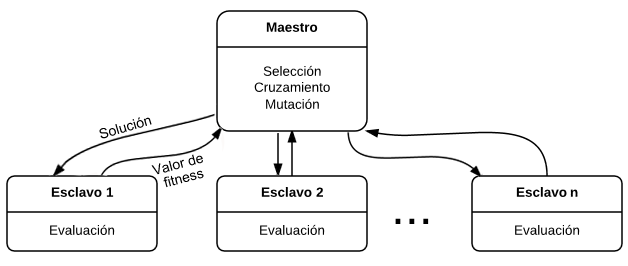
\includegraphics[width=0.7\linewidth]{Figures/diagrama-master-slave}
	\caption[Modelo Maestro-Esclavo]{Modelo Maestro-Esclavo}
	\label{fig:diagrama-master-slave}
\end{figure}

\subsection{Implementacion y Frameworks}

A la hora de implementar un algoritmo genético es importante tener en cuenta ciertos aspectos que dotaran a la solución de una mayor flexibilidad, eficiencia y robustez.

El paradigma de orientación a objetos aporta múltiples ventajas entre las que se encuentra: reusabilidad del código, abstracción de problemas, modularidad y legibilidad. Aunque hay que tener en cuenta que esto puede ocasionar perdidas de eficiencia computacional por lo que hay que balancear estos aspectos.

En el trabajo de \citep{Alba1997} se indican con mas detalles los elementos importantes de una implementacion, entre ellas destacamos: no utilizar tamaño fijo para las poblaciones pues afectan la flexibilidad, evitar las múltiples evaluaciones sobre una misma solución, dar al usuario la posibilidad de extender las funcionalidades de manera modular, al implementar bibliotecas genéricas usar lenguajes orientado a objetos pues permite su extensión en forma sencilla.

Por estas razones se han desarrollado \emph{frameworks} para trabajar en la resolución de problemas utilizando algoritmos evolutivos y otras técnicas heurísticas. Estos encapsulan de manera transparente al usuario los aspectos antes mencionados lo que permite un desarrollo mas rápido, sencillo y seguro.

Existe una gran variedad de \emph{frameworks}, a continuación se describen algunos de los mas populares junto con sus principales características.

\begin{itemize}
	\item JMetal: Es un \emph{framework} orientado a objetos basado en java para la optimización de problemas multiobjetivo utilizando metatarsianas. Su arquitectura permite tanto experimentar con técnicas provistas o desarrolladas por el usuario. Entre sus características destacan que al ser en Java puede ser usado tanto en sistemas Windows como Linux. Posee una amplia variedad de algoritmos multiobjetivo listos para usar, y también algoritmos paralelos. Está en constante desarrollo y posee una documentación detallada.\citep{Jmetal}
	
	\item Galib: Es una librería escrita en c++ que incluye objetos y herramientas útiles para la resolución de problemas usando algoritmos genéticos. Es gratuita y de código abierto, pudiendo ser ejecutada tanto en Linux como en Windows. No tiene un desarrollo sostenido siendo su última actualización en el año 2000, esto no quita que todavía se siga usando por su sencillez y flexibilidad. \citep{Galib}
	
	\item Paradiseo: Es un \emph{framework} orientado a objetos que utiliza C++. Su objetivo es el diseño de metaheurísticas tanto paralelas como distribuidas. Cuenta tanto con algoritmos evolutivos, búsquedas locales y optimización basado en enjambres. Funciona tanto en plataformas Windows como Linux y posee varios módulos destinados a extender sus funcionalidades. Tiene una buena documentación y su ultima versión data del año 2012. \citet{Paradiseo}
	
	\item Open Beagle: Es un \emph{framework} en C++ utilizando algoritmos evolutivos. Brinda un entorno de alto nivel para trabajar con distintas técnicas, soportando programación evolutiva, algoritmos genéticos y estrategias evolutivas. Su arquitectura permite utilizar los principios de la programación orientada a objetos para lograr un código recusable y eficiente. Sus características apuntan a brindar un entorno amigable, eficiente, multi-plataforma y gratuito. \citep{OpenBeagle}
	
	\item Mallba: Es una biblioteca escrita en c++ que brinda esqueletos de algoritmos para la resolución de problemas de optimización tanto exactos, heurísticos como híbridos. Maneja el paralelismo de forma simple para el usuario. Posee una arquitectura flexible y extensible lo que permite agregar nuevos esqueletos de forma simple. No cuenta con documentación extensa pero si con varios ejemplos completos de implementaciones de los algoritmos. Funciona tanto en ambiente Linux como Windows, pero se dejó de actualizar en el año 2002 por lo que es posible que no funcione correctamente en entornos mas modernos. \citep{Mallba}
	
	\item Malva: Surge como un derivado de la biblioteca Mallba con modificaciones para ser ejecutado en ambientes actuales, por lo que cuenta con las mismas características aunque al estar en fase de desarrollo soporta solo algunos algoritmos entre ellos algoritmos genéticos. \citep{Malva}
\end{itemize}

Los \emph{frameworks} son una herramienta importante a la hora de desarrollar un algoritmo evolutivo. Si nos enfocamos en la sincronización de semáforos también serán necesarias otras utilidades entre las que se encuentra los simuladores de tráfico, los cuales serán explicados en la siguiente sección.


\section{Simulación de tráfico}

Los simuladores de tráfico son programas que simulan el movimiento del flujo vehicular sobre una red, cabe destacar que esta puede ser tanto terrestre, marítima o aérea. Son usados en proyectos de investigación , estudio de congestiones y análisis de impacto de obras.  Existen varias razones para optar por esta herramienta, como es la rapidez en la obtención de resultados ya que la simulación se puede realizar en tiempos mucho más rápidos que en la realidad, el costo pues no es necesario cambiar la infraestructura para probar nuevos escenarios y es útil para prever situaciones que podrían darse bajo determinadas circunstancias.

Los simuladores se pueden dividir en dos grandes categorías, macroscópicos y microscópicos. En algunos casos se considera una tercera categoría híbrida de estas dos llamada mesoscópicos.

\begin{itemize}
	\item Macroscópicos: El tráfico es modelado como un fluido continuo y es descrito de manera agregada usando características como la velocidad o densidad del flujo.
	\item Microscópicos: El tráfico se considera compuesto de partículas discretas. Cada una es actualizada según las propiedades de la red en ese momento, como limites de velocidad, vehículos cercanos y caminos a seguir. Utilizan un modelo de decisiones del conductor, esto permite crear una distribución heterogénea del comportamientos de vehículos.
	\item Mesoscópicos: En general representa a los individuos con alto nivel de detalle pero sus interacciones y actividades con un bajo nivel de detalle.Por ejemplo agrupando vehículos en paquetes que se mueven por una red, considerándolos como una sola entidad.
\end{itemize}

En general se considera que las simulaciones microscópicas se acercan mas a la realidad y que obtienen un nivel de granularidad mayor. Esto puede ser útil cuando se asignan propiedades sobre cada vehículo y se quiere observar el comportamiento cuando estas cambian. Esto no implica que se dejen de usar simulaciones macroscópicos pues aunque no poseen tanto detalle si son mas rápidas y en determinadas circunstancias podrían ser una mejor opción.

En el trabajo de \citet{review_trafico} se puede encontrar detalles y descripción de varios simuladores entre los que se encuentran:
\begin{itemize}
	\item \citet{SUMO}: Simulador abierto, portable, microscópico diseñado para soportar grandes redes de tránsito. Es de los más populares, utiliza una serie de archivos de configuración para representar las rutas, los vehículos y el tráfico.
	\item QuadStone Paramics Modeller: Simulador modular y microscópico capaz de modelar un amplio rango de problemas de tránsito y transporte.
	\item Aimsun: Paquete de simulación que integra varios tipos de modelos de transporte, por ejemplo herramientas para el tráfico estático y un simulador microscópico
	\item Trafficware SimTraffic: Es un simulador que forma parte del paquete \emph{Trafficware's Syncro Studio}, que cuenta con una herramienta para la sincronización de semáforos.
	\item Corsim Trafvu: Parte del paquete \emph{Tsis Corsim}, presenta las animaciones y los gráficos estáticos para las redes de tráfico utilizando \emph{Corsim} como entrada.
\end{itemize}


\begin{figure}[H]
	\centering
	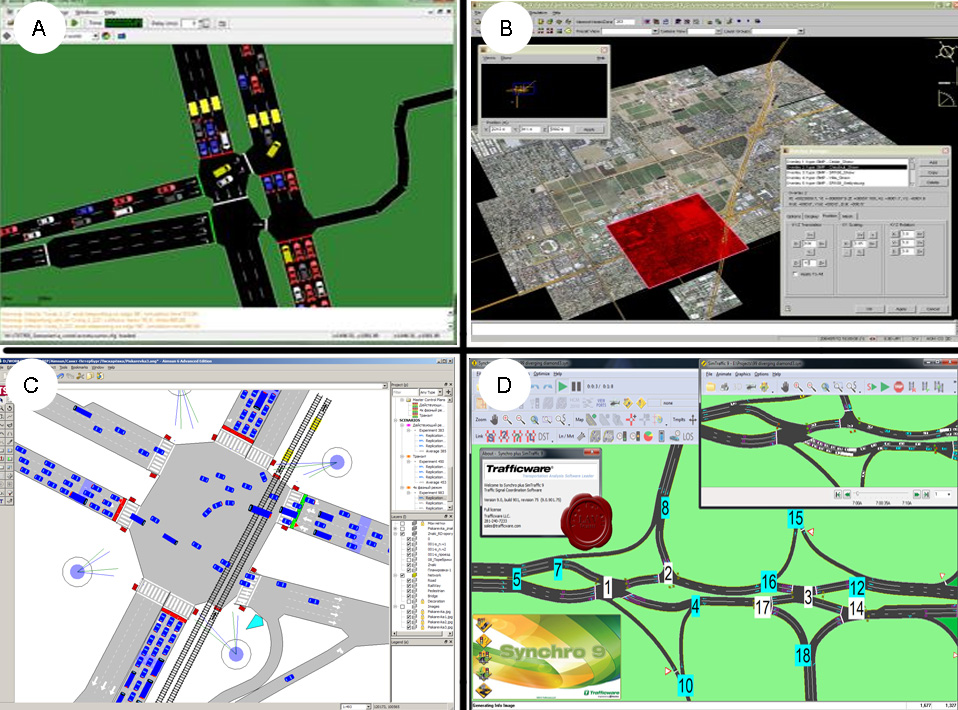
\includegraphics[width=0.7\linewidth]{Figures/simuladores}
	\caption[]{Algunos simuladores de tráfico. (A) Sumo, (B) QuadStone Paramics, (C) Aimsun, (D) Trafficware SimTraffic}
	\label{fig:simuladores}
\end{figure}

Los simuladores requieren la creación de una \emph{red de transito}, en general se refiere a las propiedades que tendrán los caminos, por ejemplo cantidad de carriles, limite de velocidad, ubicación, largo, conexiones entre las mismas, etc. Algunos simuladores obtienen esta entrada usando archivos de texto, lo cual puede ser un proceso lento y propenso a errores, otros pueden importar redes de diversas fuentes como \citet{OSM}.

También necesitan conocer las\emph{ rutas seguidas por los vehículos}. Los simuladores pueden tomar esta información de manera explicita indicando para cada vehículo la ruta seguida o utilizar otros métodos dinámicos indicando solo los puntos de inicio y final del recorrido cuya ruta será generada en tiempo de simulación. Esto puede ser un proceso verdaderamente complejo por tal razón muchos simuladores poseen herramientas destinadas a facilitar esta tarea.

Un aspecto importante a tener en cuenta es la salida que genera el simulador, ya que es fundamental a la hora de sacar conclusiones. En general la información básica sera la velocidad y tiempos de recorrido. Aunque también puede contener mas detalle como: duración de detenciones, densidad de tráfico, uso de combustible o cantidad de emisiones contaminantes.  
 


\section{Trabajos relacionados}

La investigación del estado del arte se realizó con dos objetivos en mente, el primero analizar las distintas soluciones que existen actualmente para el problema y segundo encontrar nuevas prácticas, algoritmos o utilidades que pudieran fortalecer la solución.

El problema del tráfico optimizando las luces de los semáforos se puede resolver por diferentes métodos como  redes neuronales \citep{Lopez1999}, lógica difusa \citep{Lim2001}, redes de petri \citep{DiFebbraro2002}, etc; por lo tanto la cantidad de soluciones encontradas fue abundante y variada, por esto se decidió enfocarse en soluciones cercanas a la propuesta y en otras que tuvieran alguna particularidad interesante para destacar.


\begin{itemize}
	\begin{item}
		\bibentry{Sanchez2004}
		
		Este trabajo se basa en tres puntos: El uso de algoritmos genéticos para la optimización, simulación de autómatas celulares para la función de evaluación del tráfico y un cluster para realizar ejecuciones en paralelo.
		El modelo es pequeño con 5 calles de 2 vías que se intersectan.
		La codificación del cromosoma es un vector de números enteros, donde se codifica para cada intersección cual calle está habilitada en cada ciclo.
		Usa una estrategia de selección elitista donde los dos mejores se clonan a la siguiente generación y el resto es generado por cruzamiento de dos puntos.
		
		Para la evaluación se utiliza el tiempo que transcurre desde el momento que un vehículo entra en la red hasta que sale. Se utilizó un cluster y programación paralela con una estrategia maestro-esclavo, el maestro envía los cromosomas a los esclavos que evalúan y devuelven el resultado, luego el maestro se encarga de generar la siguiente población.
		
		Se compararon los resultados con una simulación aleatoria y con una fija, obteniendo la solución propuesta mejores resultados en todos los casos evaluados.
		
		Este mismo grupo realizó trabajos similares expandiendo esta investigación, que se presentan a continuación.
	\end{item}
	
	\begin{item}
		\bibentry{Sanchez2008}
		Lo interesante de este estudio es que se aplica lo expuesto en el trabajo anterior a un lugar real en Santa Cruz de Tenerife para validar los resultados.
		Algunas mejoras que se introdujeron fueron que el cromosoma se codifica utilizando código Gray lo que dicen mejora el rendimiento en mutación y cruzamiento. La población inicial esta compuesta por nueve \emph{soluciones} provistas por la alcaldía de la ciudad. Tanto la estrategia de selección como de cruzamiento y mutación es similar al anterior trabajo.
		
		El modelo se discretizó en 42 semáforos, 26 entradas y 20 salidas.
		Las soluciones provistas por la alcaldía se simularon y se utilizó para comparar con los resultados obtenidos por el algoritmo que en términos generales logra una mejora de hasta 26\%.
		
	\end{item}
	
	\begin{item}
		\bibentry{Sanchez2010}
		Este trabajo es similar al anterior pero se destacan algunos cambios, por ejemplo se probaron cuatro funciones de fitness diferentes, ellas fueron: cantidad de vehículos que llegaron a destino, tiempo de viaje promedio, tiempo de ocupación promedio y velocidad promedio global.
		También agrega medidas correspondientes al gas total emitido por los vehículos que tiene relación con la velocidad a la que van.
		El modelo discretizado de la zona de \emph{La Almozara} cuenta con 17 semáforos, 7 intersecciones, 16 entradas y 18 salidas.
		Se simuló tanto un caso standard como casos de alta congestión de tráfico, las comparaciones se hacen respecto a las distintas funciones de fitness y los distintos escenarios planteados logrando buenos resultados.
		
	\end{item}
	
	
	\begin{item}
		\bibentry{Penner2002}
		Este trabajo se centra en un modelo de simulación basado en enjambres que luego se optimiza utilizando un algoritmo genético cuya función de fitness es el tiempo promedio de los vehículos dentro de la red. El cromosoma cuenta con la secuencia y duración de los semáforos, así como la relación con los semáforos complementarios, la mutación tiene en cuenta esto para que no ocurra en una misma intersección dos luces verdes. El cruzamiento se hace entre los distintos semáforos con una probabilidad más alta si esta en la misma intersección.
		
		El primer escenario es pequeño, cuenta con una ruta de 3 carriles y 3 intersecciones.Con diferentes variaciones logra mejoras significativas.
		
		Luego se realiza otro escenario más complejo de 28 semáforos y 9 intersecciones logrando mejoras de hasta 26\%.
	\end{item}	
	
	
	\begin{item}
		\bibentry{Stolfi2012}
		Este trabajo se basa en el concepto de una ciudad inteligente enfocado en la movilidad, indica que los atascos del tráfico provocan tanto perdidas económicas como también contaminación ambiental.
		
		Utiliza un algoritmo inteligente que tomando en cuenta el estado de congestión de las rutas sugiere al usuario cual es la ruta más rápida a su destino, utilizando un dispositivo en el automóvil que se enlazara por \emph{wifi} con los semáforos que cuentan con sensores. Por lo tanto el trabajo no se basa en la optimización de las señales de los semáforos existentes sino agrega encima de esto un sistema de búsqueda de mejor ruta.
		
		Para el modelo utiliza una zona  de la ciudad de Málaga, cuenta con 8 entradas y 8 salidas, para la simulación utiliza \citet{SUMO}. Los vehículos modelados son: turismo, monovolumen, furgoneta y camión donde se varía la longitud, velocidad y probabilidad que entre en la red de tráfico.
		
		Se intenta minimizar los tiempo de viaje de los vehículos que circulan por la red. Para ellos se utiliza un algoritmo genético cuya estrategia de selección consiste en tomar los dos peores individuos reemplazándolos por los dos mejores hijos encontrados. En el cromosoma se representa cada sensor, con los destinos y rutas posibles. La función de fitness tiene en cuenta la cantidad de viajes completados durante el tiempo de ejecución, el tiempo medio utilizado y el retraso medio. Se prueban varias estrategias de cruzamiento y mutación. Las ejecuciones tienen un tiempo fijo de duración.
		
		
		Compara el resultado con una simulación donde se generaron 64 itinerarios diferentes, esto se prueba en 3 escenarios. Las simulaciones se realiza hasta con 800 vehículos, concluyendo que al aumentar la cantidad de vehículos (más de 400) en el sistema la solución mejora sustancialmente el resultado base.
		
	\end{item}	
	
	
	\begin{item}
		\bibentry{Teo2010}
		Este trabajo presenta un modelo simple con una sola intersección en donde se intenta optimizar los tiempos de los semáforos para lograr mejorar rendimiento del tráfico. El cromosoma representa los tiempos de la luces verdes mientras que la función de fitness es el largo de las colas generadas. Un aspecto interesante es que la simulación tiene un tiempo fijo de 600 segundos por generación pero no se detalla el tipo de simulación utilizada. Las conclusiones indican que la optimización usando algoritmos genéticos  es buena para el problema del flujo de tráfico.	
	\end{item}	
	
	
	\begin{item}
		\bibentry{Montana1996}
		Esta propuesta utiliza un enfoque adaptativo con sensores que analizan el tráfico en tiempo real. Un sensor para saber cuantos autos pasan y otro para saber que tan larga es la cola. Considera los cambios que se producen con respecto al caso promedio y cambia los tiempos de las señales en forma acorde.
		La premisa se basa en la inteligencia colectiva en donde agentes individuales realizan tareas simples que al interactuar producen resultados globales.
		
		Se aplica programación genética más específicamente STGP (strongly typed genetic programming) \citep{Montana1995} que aprende el árbol de decisión que será ejecutado por todas las intersecciones cuando decida el cambio de fase. Además un algoritmo genético híbrido busca diferentes constantes que serán usadas en los arboles de decisión mejorando el flujo de tráfico.
		
		La medida básica de efectividad en la función de evaluación es el \emph{Delay}, esto es el total de tiempo perdido por causa de las señales de tráfico. Se probaron tres modelos distintos de cuatro intersecciones con una versión especial del simulador  TRAF-NETSIM \citep{TRAF-NETSIM}
		
		El experimento arroja buenos resultados en cuando a la performance de la red y destaca la buena adaptabilidad en diferentes circunstancias. Aunque se marca el hecho de que el modelo es simple y de tamaño pequeño, siendo una incógnita como funcionara con problemas más complejos.
		
	\end{item}	
	
	
	\begin{item}
		\bibentry{Vogel2000}
		
		La solución utiliza un enfoque auto-adaptable para mejorar el tráfico tanto en el corto como en el largo plazo a través de la optimización de las señales de tráfico en las intersecciones de una red de rutas. Al darle dinamismo a cada intersección se mejora el rendimiento de la red.
		
		Destaca el hecho que dada una configuración de semáforos aún siendo optimizada usando simulaciones es difícil que sea la mejor en todas las situaciones o en casos extremos (horas picos). Para solucionar esto proponen un sistema auto-adaptable que toma la información del tráfico actual usando detectores de vehículos y espacios.
		
		Utiliza el concepto de fases para representar las distintas posibilidades en la señalización de la intersección y cuanto tiempo debe permanecer en esa fase. 
		Propone el desarrollo de un algoritmo evolutivo donde cada individuo representa un sistema de fases mientras el fitness se obtiene simulando ese sistema en un modelo de tráfico. Este es relativamente pequeño con una intersección con cuatro brazos, cada uno con tres líneas donde la ruta principal tiene el doble de densidad vehicular. 
		
		Los resultados indican que la ventaja de usar conocimiento experto para configurar los parámetros iniciales es mínimo ya que llega muy rápido a resultados similares. Tanto la búsqueda de los mejores parámetros como en estructuras más simples el algoritmo se comporta con buenos resultados.
		
	\end{item}	
	
	\begin{item}
		\bibentry{Rouphail2000}
		
		Se estudia una pequeña red de tráfico de nueve intersecciones con semáforos en la ciudad de Chicago, contando con tráfico de vehículos, parking, rutas de ómnibus y paradas.  
		Se toman valores reales en horas pico, comprobando que las colas que se generan en la simulación coinciden con la realidad.
		Usa el programa \citep{TRANSYT-7F} que permite visualizar mapas y contiene optimización de varios algoritmos genéticos y \citep{CORSIM}  un simulador de tráfico comercial.
		Se probaron 12 estrategias distintas de resolución midiendo el tiempo de demora en la red y el largo de las colas producidas. Los resultados indican que la performance de la red aumentó considerablemente usando este método.	
	\end{item}	
	
\end{itemize}


\subsection{Resumen}
Aquí un breve repaso sobre los trabajos evaluados y su comparación con la propuesta presentada.

El trabajo de \citet{Sanchez2004} posee algunos puntos de contacto como es la ejecución paralela en un cluster y la arquitectura maestro-esclavo. La principal diferencia es que el escenario que evalúan es pequeño y no se compara con un escenario real.

El siguiente trabajo de \citet{Sanchez2008} expande lo anterior y lo utiliza en un caso real en Santa Cruz de Tenerife siendo de una complejidad similar a Garzón en términos de cantidad de cruces y semáforos. Los resultados obtenidos son muy positivos obteniendo mejoras de hasta 26\%.

Se destaca de \citet{Sanchez2010} las pruebas de diferentes funciones de fitness teniendo en cuenta diversos factores como tiempo de viaje o velocidad promedio. Este trabajo inspiro la realización de una función multiobjetivo que tuviera en cuenta la velocidad promedio en el proyecto actual.

Aunque \citet{Stolfi2012} no optimiza la configuración de los semáforos, si plantea una posibilidad interesante para mejorar el tráfico en una ciudad indicando a los vehículos la mejor ruta por lo que se podría tomar como un elemento en trabajos futuros.

Tanto los trabajos de \citet{Teo2010} como \citet{Stolfi2012} plantean la simulación con un tiempo fijo lo que se utilizó en el proyecto.

\citet{Montana1996} y \citet{Vogel2000}  proponen algoritmos que se adapten en tiempo real por lo que se destacan como posibles trabajos a futuro.
Es digno de mención que todos los trabajos consultados lograron mejoras significativas en sus resultados.

En conclusión el estudio de los trabajos relacionados permitió conocer en profundidad distintas soluciones y métodos que fueron tenidos en cuenta en menor o mayor medida en la solución propuesta. El hecho de que se obtuvieran buenos resultados motivo aún más el desarrollo del trabajo presentado.





